\providecommand{\main}{../../../..}
\documentclass[\main/dresen_thesis.tex]{subfiles}

\begin{document}
  \paragraphNewLine{Scanning Electron Microscopy}
    The drop casted monolayers ML-Ac-CoFe-C and ML-Ac-CoFe-C-2 have both been characterized in top view with SEM micrographs at varied magnifications measured with a Neon Zeiss 40 (\refsec{ch:instruments:laboratoryInstruments:sem}).
    Furthermore, cross-sectional views in SEM of the monolayer ML-Ac-CoFe-C have been obtained by cutting the sample with a diamond cutter and subsequently breaking it.
    For ML-Ac-CoFe-C-2, the sample has not been broken but instead an equivalent sample that has been prepared in parallel from the same dispersion, under the same conditions, is broken and viewed in SEM.
    The micrographs are measured at $5 \unit{kV}$ and the shown micrographs are measured by the back scattering electron detector.

  \paragraphNewLine{Reflectometry}
    Both samples ML-Ac-CoFe-C and ML-Ac-CoFe-C-2 have been measured with XRR using a Bruker D8 Advanced at the \textsc{Forschungszentrum J\"ulich} (\refsec{ch:instruments:laboratoryInstruments:xrr}).
    A $q$-range of $0 \ldots 0.4 \unit{\angstrom^{-1}}$ has been measured by using the equipped Cu-K$\alpha$ source ($\lambda \eq 1.54 \unit{\angstrom}$) and measuring an angle range of $2 \theta \eq 0 \ldots 3 \unit{^\circ}$ in $0.005 \unit{^\circ}$ steps over an integrated time of approximately $1 \unit{h}$.
    For footprint correction (\refsec{ch:methods:xrr}), the beam width is estimated by the size of the collimation slits, which is $0.2 \unit{mm}$, and the samples both have a width of $10 \unit{mm}$.

    Furthermore, neutron reflectometry was measured for ML-Ac-CoFe-C at the D17 instrument in the Institute Laue-Langevin (\refsec{ch:lss:d17}).
    D17 was operated in time-of-flight (TOF) mode and a $q$-range of $0 \ldots 0.2 \unit{\angstrom^{-1}}$ was obtained by measuring the reflectivity for the three incident angles $\alpha_i \eq 0.50^\circ ,\, 1.80^\circ ,\, 4.00^\circ$.
    As the measurement was performed in TOF mode, no footprint correction needs to be applied.
    For data reduction and estimation of the instrumental resolution the COSMOS software is used, which is maintained by the instrumental scientists \cite{Gutfreund_2018_Towar}.
    The data used for the discussion of the nuclear structure of the monolayer, was obtained after zero-field cooling at $\mathrm{T} \eq 5 \unit{K}$ with polarized neutrons at a guide field of $B \eq 10 \unit{mT}$.

    \begin{figure}[tb]
      \centering
      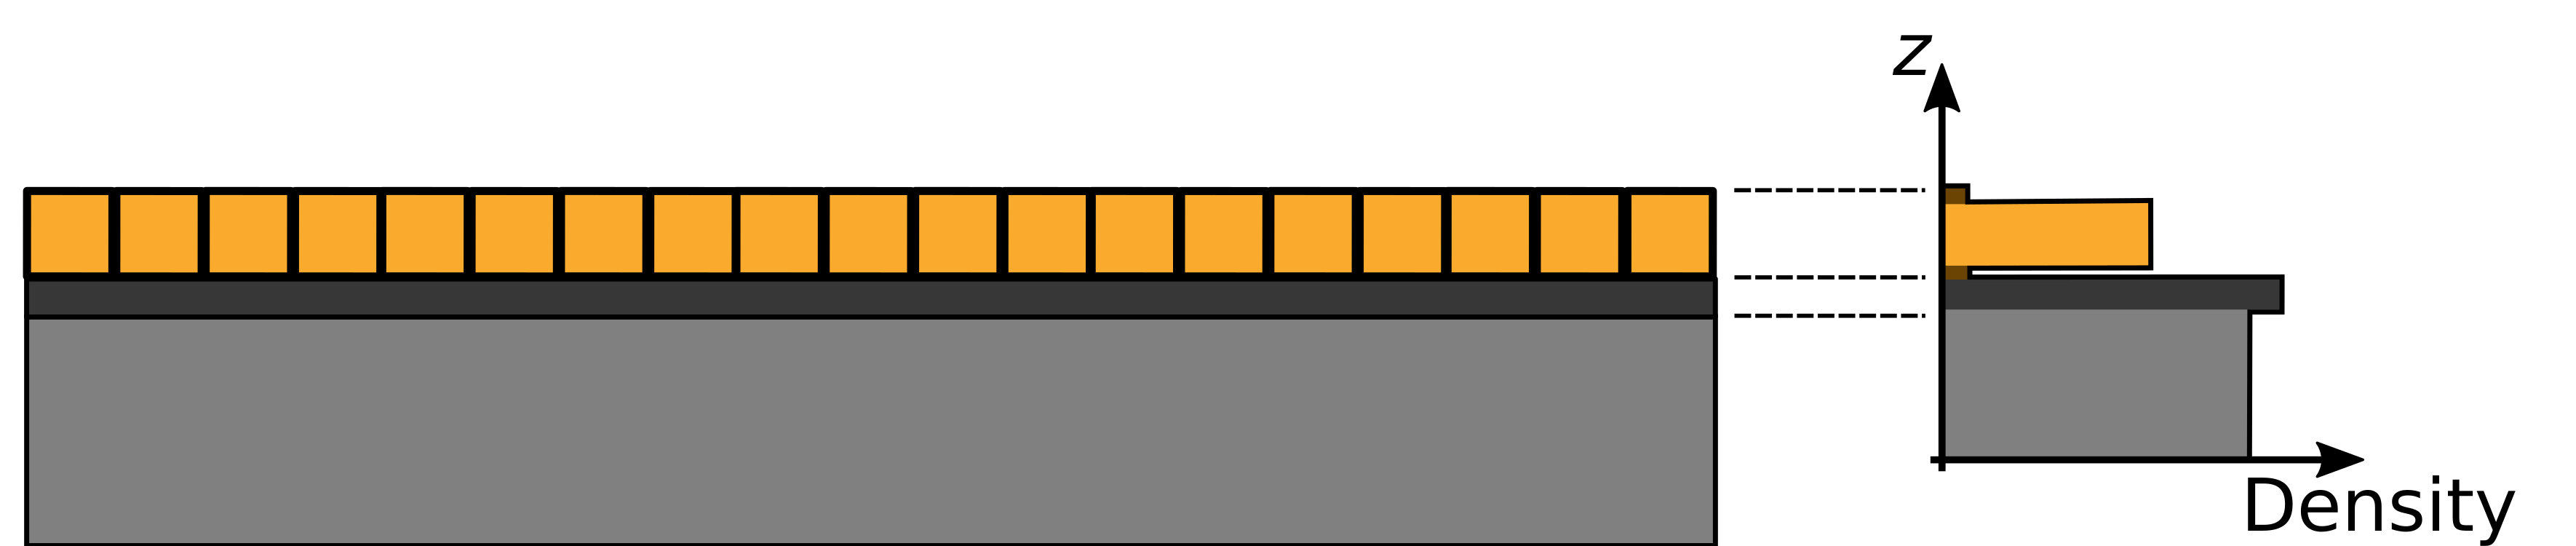
\includegraphics{monolayers_structure_verticalModel}
      \caption{\label{fig:monolayers:structure:verticalModel}Model for a square array of nanocubes depicted as cartoon of the cross-section (left) and the expected resulted shape of the vertical density structure (right). The sample can be modeled by a layered system of silicon (light gray), silicon dioxide (dark gray), oleic acid (brown) and cobalt ferrite (orange). }
    \end{figure}

    The obtained reflectivities are discussed by using the model that is schematically depicted in \reffig{fig:monolayers:structure:verticalModel}.
    The substrate is set to be silicon with a layer of silicon dioxide on top.
    The average lateral density of a square array layer is modeled by a single slab of nanocubes (NC), with oleic acid (OA) slabs around it.
    And at last, which is not depicted in \reffig{fig:monolayers:structure:verticalModel}, the interfaces are not clear cuts in the vertical plane, but have an interfacial roughness, which are included by Névot-Croce roughness factors in the model for each interface.

    In total this model has $4$ parameters to describe the thickness of the nanocubes, the two OA and the \ch{SiO2} layers and $5$ roughness parameters for the interfaces \ch{Si}/\ch{SiO2}, \ch{SiO2}/OA, OA/NC, NC/OA  and OA/air.
    Additionally it has $4$ parameters to describe the SLD of silicon, the \ch{SiO2}, the nanocubes and the OA.
    The edge length of the nanocubes has been determined by small-angle scattering experiments and is therefore fixed.
    And the scattering length densities of the materials are fixed to the literature values, where for X-rays the imaginary part of the scattering length density is included to account for absorption by cobalt ferrite.
    The used scattering length densities are tabulated in \reftab{tab:monolayers:charMethod:reflectometryScatteringLenghts}.
    For the NC layer a packing density factor $\eta$ is multiplied to the scattering length density to account for the particle spacing.
    The model totals therefore to $9$ refined parameters.

    \begin{table}[ht]
      \centering
      \caption{\label{tab:monolayers:charMethod:reflectometryScatteringLenghts}Scattering length values fixed in the calculation of the reflectivity. For XRR the electronic SLD $\rho_\mathrm{el.}$ is calculated for Cu-K$\alpha$ ($\lambda \eq 1.54 \unit{\angstrom}$) and for NR the nuclear SLD $\rho_\mathrm{nuc.}$ is used \cite{Sears_1992_Neutr, BerkeleyLab_1993_asf}.}
      \begin{tabular}{ l | c | c }
        \textbf{SLD}  & $\rho_\mathrm{el.} \, / \unit{10^{-6} \angstrom^{-2}}$ & $\rho_\mathrm{nuc.} \, / \unit{10^{-6} \angstrom^{-2}}$ \\
        \hline
        $\ch{Si}$                                 & $20.122 - 0.459 i$   & $2.079$  \\
        $\ch{SiO2}$                               & $22.724 - 0.294 i$   & $4.186$  \\
        Oleic Acid ($\ch{C18H34O2}$)              & $8.520  - 0.013 i$   & $0.078$  \\
        Ac-CoFe-C ($\ch{Co_{0.66}Fe_{2.22}O4}$)   & $39.445 - 3.663 i$   & $6.194$  \\
        Ac-CoFe-C-2 ($\ch{Co_{0.8} Fe_{2.13}O4}$) & $39.963 - 3.749 i$   & $6.135$  \\
        \hline
      \end{tabular}
    \end{table}

    % Additional to the described model property parameters, instrumental parameters are included in the model: the instrumental resolution needs to be considered either by including angular divergence and energy resolution or by using the resolution function that is known from the instrument.
    % Also as the sample alignment has finite precision, a small linear shift in $q$ is allowed in the model.

    The parameter values are refined by applying the Levenberg-Marquardt algorithm \cite{Marquardt_1963_Analgo}, to minimize the figure of merit $\mathrm{FOM}$, which is defined here for reflectometry as a $\chi^2$ function on the logarithmic scale
    \begin{align}
      \mathrm{FOM} \eq \sum_{q_i} \biggl( \log(I) - \log(I_\mathrm{model})\biggr)^2.
    \end{align}
    Due to the strong weight of the reflectivity in the small-$q$ range, the errorbars are ignored for the refinement to focus the algorithm on finding a model that describes the whole dynamic range properly.

    From the refined packing density, the relative particle spacing $a_{p-p}$ is estimated by assuming that the measured surface is fully covered by square lattice of nanocubes with SLD $\rho_\mathrm{NC}$ and the particle spacing is filled with oleic acid of SLD $\rho_\mathrm{OA}$ and thus
    \begin{align}
      \label{eq:monolayers:characterization:particleSpacing}
      \begin{split}
        &\eta \rho_\mathrm{NC}  \eq \frac{a^2}{a_{p-p}^2} \rho_\mathrm{NC} + \frac{a_{p-p}^2 - a^2}{a_{p-p}^2} \rho_\mathrm{OA},\\
        \Rightarrow& a_{p-p} \eq a \sqrt {\frac{\rho_\mathrm{NC} - \rho_\mathrm{OA} }{\eta \rho_\mathrm{NC} - \rho_\mathrm{OA}}}
      \end{split}
    \end{align}

    \paragraphNewLine{Grazing-Incidence Small-Angle Scattering}
      The sample ML-Ac-CoFe-C-2 has been measured by GISAXS by using the GALAXI instrument (\refsec{ch:lss:galaxi}) ($\lambda \eq 1.34 \unit{\angstrom}$).
      The incident angle was chosen to $0.15 ^\circ$ at a sample-to-detector distance of $1.733 \unit{m}$.
      An initial evaluation of the GISAXS is performed analogue to the discussion of the GISAXS detector images obtained for the samples from solvent variation in \refsec{sec:monolayers:nanoparticle:dropcastingExperiments} by fitting a Voigt function to the first order peak in the Yoneda band.
      From the fitted parameters, the lattice constant $a$, coherence length $L_\mathrm{coh.}$ and uncertainty of the nearest neighbour position $\sigma_\mathrm{n.N.}$ is estimated.

      For a more precise investigation of the grazing-incidence scattering, the BornAgain software package \cite{Burle_2018_borna} is used to simulate the two dimensional detector data by the model of nanocubes with a paracrystalline square lattice interference function.
      The edge length, it's size distribution and the scattering length density of the nanocubes are set to the values obtained from the nanoparticle characterization by small-angle scattering in \refsec{sec:monolayers:nanoparticles}.
      Similar to the vertical structure model, it is assumed the sample is a multi layer structure with a \ch{Si} substrate, a \ch{SiO2} intermediate layer and the nanocubes sit within an oleic acid layer.
      As layer thickness, the same values as in XRR and the SLD of the layers are calculated from literature using the GALAXI wavelength of $1.34 \unit{\angstrom}$ for each material respectively.
      The Gaussian broadening is included to simulate the instrumental resolution of GALAXI.
      In the simulation, it is assumed that the orientation of the lattice is on average random with respect to the beam and the probability functions of the position uncertainty in the square lattice paracrystal are assumed to be Gaussian functions.

  \paragraphNewLine{Polarized Neutron Reflectometry}
    % Polarized neutron reflectometry has been performed on SuperADAM at the ILL for all discussed samples at a temperature of $300 \unit{K}$ and at a low temperature of $30 \unit{K}$.
    % The distance between sample and detector for the experiments was $2.009 \unit{m}$ and a range of incident angles from $0 ^\circ \ldots 3 ^\circ$ is measured.
    % The neutron wavelength was selected to $\lambda \eq 5.14 \unit{\angstrom}$ and $\lambda \eq 5.18 \unit{\angstrom}$ for the measurements at $300 \unit{K}$ and $30 \unit{K}$ respectively.
    % The wavelength spread is in both cases $0.5 \%$ (FWHM) as provided by the instrumental scientists.
    % The monochromator aperture is set to $1 \unit{mm}$ and the sample aperture to $0.5 \unit{mm}$ along the scattering direction for the measurements at $300 \unit{K}$, and to $3 \unit{mm}$ and $1 \unit{mm}$ for the measurements at $30 \unit{K}$.

    % At room temperature, the samples are fixed by a vacuum suction and measured at a guide field of $4 \unit{mT}$, at a high magnetic field of $500 \unit{mT}$ and subsequently again at $4 \unit{mT}$ in remanence.
    % For the measurements at $30 \unit{K}$, the samples are fixed in a cryostat using Apiezon vacuum grease and the guide field is measured to be $2.4 \unit{mT}$.
    % The procedure is in each case to cool the samples from room temperature to $30 \unit{K}$ at guide field and measure the initial reflectivity.
    % Then the reflectivity is measured at an applied field of $730 \unit{mT}$, and subsequently in remanence at guide field again.
    % To study the reflectivity after field-cooling, the samples are heated above $200 \unit{K}$ and cooled back to $30 \unit{K}$ at an applied field of $730 \unit{mT}$.
    % The reflectivity is then measured at the applied field and finally in remanence of the field-cooled state.

    % For the room temperature measurements, a range of incident angles from $0^\circ \ldots 3 ^\circ$ is measured in $0.01 ^\circ$ steps with $20 \unit{s} - 60 \unit{s}$ counting time, with an linear increase with respect to the incident angle.
    % In the $30 \unit{K}$ measurements, the range is increased to $4 ^\circ$ and the counting time is increased non-linearly in the range from $4 \unit{s} - 200 \unit{s}$ in accordance to the asymptotic behaviour of Fresnel's reflectivity, which drops in intensity with $q^4$.

    % All measurements are performed with polarized neutrons, providing two reflectivity channels for each measurement, one for neutrons parallel to the magnetic field direction, and one for neutrons that are anti-parallel.
    % For the layers prepared from IOS-11, an additional polarization analysis is performed for the low-temperature measurements to measure the spin-flip channel of neutrons coming from an anti-parallel incident state and are outgoing in a parallel state.
    % For the remaining samples, no polarization analysis is performed.
    % The polarization efficiency is measured from the direct beam to be $\approx 99 \%$ at guide field and high field.

    % The detector images are scaled to it's respective monitor to correct for varying counting-times and fluctuating incident beam intensities.
    % Due to a malfunction of the monitor for the field-cooled remanence measurement of 8BL-15-IOS-11, this specific measurement is scaled to the counting time instead.
    % The detector images are reduced by integrating the detector dimension perpendicular to the scattering plane, providing a intensity map with respect to the incident angle and remaining detector dimension for each measurement and each channel.
    % The coordinates are transformed to ($\alpha_i - \alpha_o$, $\alpha_i + \alpha_o$) using the pixel-splitting rebinning algorithm described in \refapp{ch:appendix:numericalMethods:rebinningPixelSplitting}.
    % To obtain the reflectivity curves, a box in the range $\alpha_i - \alpha_o \eq -0.1 ^\circ \ldots 0.1 ^\circ$ is integrated, and the diffuse scattering is subtracted with the box integrals of the ranges $\alpha_i - \alpha_o \eq \pm (0.1 \ldots 0.2)$ in the intensity map.

    % The same model as in XRR is used to describe the nuclear structure of SC-IOS-11 and SC-IOS-7.
    % The particle geometry and scattering length densities are used as obtained from SAS, and only the layer positions and packing densities are varied.
    % For the evaluation of the reflectivity curves measured for polarized neutrons $R^{+}$ and $R^{-}$, the formalism presented by Zabel \etal in \cite{Kronmueller_2007_Handb} is implemented, where the reflectivities are evaluated by
    % \begin{align}
    %   \label{eq:looselyPackedNP:pnrReflectivityFormula}
    %   R^\pm \eq \frac{1}{2} \biggl[ R_{+} \bigl(1 \pm P \cos(\gamma) \bigr) + R_{-} \bigl(1 \mp P \cos(\gamma) \bigr) \biggr].
    % \end{align}
    % Here $R_\pm$ are the reflectivities calculated for the scattering length densities $\rho_\mathrm{nuc} \pm \rho_\mathrm{mag}$, $P$ is the polarization efficiency of the instrument and $\gamma$ the angle between the sample magnetization and the neutron polarization.
    % The samples that show magnetic contrast are discussed with regard to being homogeneously magnetized such as measured in VSM, and it is studied how the agreement between the calculated and measured reflectivity changes when the magnetic density in the respective layers is allowed to be varied independently.




  \paragraphNewLine{Vibrating Sample Magnetometry}
    % Pieces from the samples SC-IOS-11 and SC-IOS-7 are studied by vibrating sample magnetometry using a PPMS Evercool II (\refsec{ch:instruments:laboratoryInstruments:vsm}).
    % Using a diamond cutter, $5 \times 5 \unit{mm^2}$ small pieces are cut and fixed on a Quartz sample holder using a low-temperature varnish (GE 7031).
    % The samples are measured at $300 \unit{K}$ over a range of $\pm 5 \unit{T}$ with a sweeping rate of $5 \unit{mT \, s^{-1}}$.
    % Furthermore, zero-field cooled and field cooled temperature-dependent magnetization measurements of both samples are performed by cooling the samples to $10 \unit{K}$ and measuring the magnetization while warming the sample with a rate of $1.5 \unit{K \, min^{-1}}$.
    % Finally, magnetization measurements at $30 \unit{K}$ are performed both after zero-field cooling and cooling in $730 \unit{mT}$.
    % For the $30 \unit{K}$ hysteresis, a range of $\pm 730 \unit{mT}$ is measured with a rate of $2.5 \unit{mT \, s^{-1}}$.

    % The magnetization data is rescaled in both cases, by performing a Langevin fit on the data obtained at $300 \unit{K}$.
    % The obtained magnetic moment is used to determine the spontaneous magnetization $M_s$ of the by assuming the particle volume as it's obtained from SAXS as described in \refsec{ch:methods:vsm} and the data is rescaled accordingly.
    % The same rescaling factor is used for the measurements at varied temperature, assuming that the magnetic volume does not change.
    % For the Langevin fit the data is corrected for the diamagnetic contribution, which is originating from the silicon substrate.


\end{document}